% Options for packages loaded elsewhere
\PassOptionsToPackage{unicode}{hyperref}
\PassOptionsToPackage{hyphens}{url}
% !TeX program = pdfLaTeX
\documentclass[12pt]{article}
\usepackage{amsmath}
\usepackage{graphicx,psfrag,epsf}
\usepackage{enumerate}
\usepackage[]{natbib}
\usepackage{textcomp}


%\pdfminorversion=4
% NOTE: To produce blinded version, replace "0" with "1" below.
\newcommand{\blind}{0}

% DON'T change margins - should be 1 inch all around.
\addtolength{\oddsidemargin}{-.5in}%
\addtolength{\evensidemargin}{-1in}%
\addtolength{\textwidth}{1in}%
\addtolength{\textheight}{1.7in}%
\addtolength{\topmargin}{-1in}%

%% load any required packages here



% tightlist command for lists without linebreak
\providecommand{\tightlist}{%
  \setlength{\itemsep}{0pt}\setlength{\parskip}{0pt}}



\usepackage{amssymb}
\usepackage{tikz-cd}

\IfFileExists{bookmark.sty}{\usepackage{bookmark}}{\usepackage{hyperref}}
\IfFileExists{xurl.sty}{\usepackage{xurl}}{} % add URL line breaks if available
\hypersetup{
  pdftitle={No More, No Less Than Sum of its Parts: The Algebra of Graphics, Statistics, and Interaction},
  pdfkeywords={Interactive data visualization, category theory, abstract
algebra, the Gestalt Principles, descriptive statistics},
  hidelinks,
  pdfcreator={LaTeX via pandoc}}



\begin{document}


\def\spacingset#1{\renewcommand{\baselinestretch}%
{#1}\small\normalsize} \spacingset{1}


%%%%%%%%%%%%%%%%%%%%%%%%%%%%%%%%%%%%%%%%%%%%%%%%%%%%%%%%%%%%%%%%%%%%%%%%%%%%%%

\if0\blind
{
  \title{\bf No More, No Less Than Sum of its Parts: The Algebra of
Graphics, Statistics, and Interaction}

  \author{
        Adam Bartonicek \\
    Department of Statistics, The University of Auckland\\
     and \\     Simon Urbanek \\
    Department of Statistics, The University of Auckland\\
     and \\     Paul Murrell \\
    Department of Statistics, The University of Auckland\\
      }
  \maketitle
} \fi

\if1\blind
{
  \bigskip
  \bigskip
  \bigskip
  \begin{center}
    {\LARGE\bf No More, No Less Than Sum of its Parts: The Algebra of
Graphics, Statistics, and Interaction}
  \end{center}
  \medskip
} \fi

\bigskip
\begin{abstract}
Interactive data visualization has become a staple of modern data
presentation. Yet, despite its growing popularity, there still remains a
lack of a formal framework for turning raw data into summary statistics
that can then be displayed by interactive graphics. This gap may stem
from a subtle yet profound issue: while we would often like treat
statistics, graphics, and interaction as independent entities, they are
in fact deeply connected. This paper aims to shed light on this
interdependence by relating it to two fundamental concepts from category
theory: groups and monoids. Specifically, if we want our graphics to
support interactive features which break the data into multiple parts
and then combine them back together (such as in the case of linked
selection), then we need the statistics in our plots to fulfill certain
algebraic properties. Ultimately, understanding this hidden structure
may empower data visualization experts to build more flexible and
expressive interactive data visualization systems.
\end{abstract}

\noindent%
{\it Keywords:} Interactive data visualization, category theory,
abstract algebra, the Gestalt Principles, descriptive statistics

\vfill

\newpage
\spacingset{1.9} % DON'T change the spacing!

\section{\texorpdfstring{Introduction
\label{sec:intro}}{Introduction }}\label{introduction}

\begin{quote}
``Effective graphical analysis makes things seem obvious, the effort
involved in making the graphical analysis effective is not so obvious.''
\citep{unwin2018}
\end{quote}

The essence of data visualization is comparison. When we visualize, we
split our data into parts, summarize each part one or more summary
statistics, encode the summaries into visual attributes such as
position, size, or color, and finally use these attributes to draw
geometric objects
\citetext{\citealp{bertin1983}; \citealp{wilkinson2012}; \citealp[for a
recent review, see][]{franconeri2021}; \citealp{wilke2019}}. For
example, when drawing a typical barplot, we split our data into parts
based on the levels of some categorical variable, count the number of
cases in each part, and finally represent the counts by drawing bars of
the corresponding heights. In this way, each bar becomes a visual
representation of its own ``small data set'', a subset of the original
data.

To ground this idea in a more concrete example that will be used
throughout this paper, imagine going through your bookshelf, sorting the
books by genre, and stacking them on top of each other. You would
construct a physical version of the barplot, forming one ``bar'' (stack)
per genre: one bar for sci-fi novels, one bar for romance, one bar for
detective fiction, and so on. Even from this very simple example,
interesting mathematical properties jump out: for example, a single book
cannot go into two stacks (the subsets of the data are \emph{disjoint})
and if all of the stacks are combined back together, we should end up
with the bookshelf we started with \citep[the subsets are
\emph{surjective} and cover the entirety of the data set,
see][]{ziemkiewicz2009}.

Now, just as we can learn about the contents of our library by
organizing books in the way we just described, we can learn about our
data by splitting it into parts. A natural question then arises: can we
learn more by subdividing our data into even smaller parts and comparing
these? For instance, in our book example, we can split each stack of
books into two smaller stacks based on the gender of the author. Each
smaller stack will then represent the unique combination (Cartesian
product) of the two categorical variables (genre and gender). Moreover,
there arises a hierarchical relationship between the stacks: by
combining two genre-gender stacks (child components) together, we can
recover the original genre stack (parent component). Similar situation
often arises in interactive graphics, where we use techniques such as
linked selection to highlight specific subsets of our data. Either way,
by forming these finer partitions, we can represent our data with
greater granularity and discover trends that may otherwise hide in the
aggregate.

However, once we have subdivided each category into its child
components, we need to represent the information in a way that visually
preserves the hierarchical nature of this relationship. In data
visualization, there are two popular methods for doing this, known as
``stacking'' and ``dodging'' (see Figure \ref{fig:playfair}). These
methods have existed at least since the time of William Playfair
\citetext{\citeyear{playfair1801}; \citeyear{playfair1822}}. Let's
briefly illustrate them on the example of the classical barplot. In a
stacked barplot, bar segments representing the product of the two factor
variables are plotted vertically on top of each other (``stacked''; the
operation can be also thought of as ``highlighting'' parts of the bar).
In contrast, in a dodged barplot, bars are plotted side-by-side, as
clusters of bars. Finally, there is also a third popular method, known
as layering, where we plot bar segments in separate graphical layers and
use partial transparency to mitigate overplotting (this technique may
have been a bit challenging for William Playfair but has been made
simple with computers).

\begin{figure}

{\centering 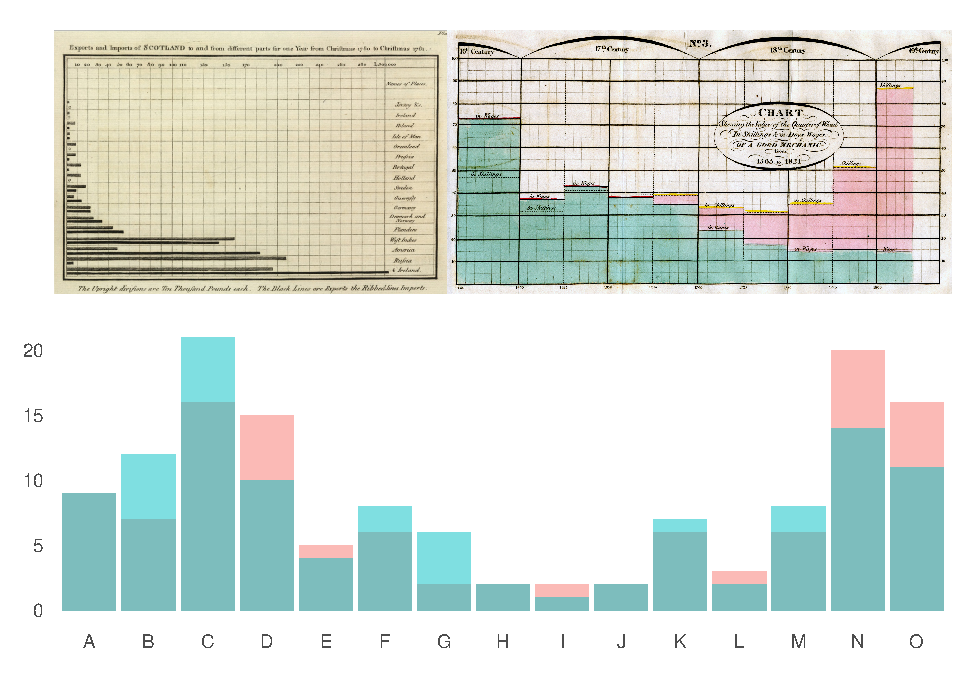
\includegraphics{paper_files/figure-latex/playfair-1} 

}

\caption{Examples of the three methods for dealing with bars that have subdivided into segments. Top row: dodging (left) and stacking/highlighting (right); both by William Playfair (1801, 1822). Bottom row: layering (created with ggplot2; Wickham, 2010).}\label{fig:playfair}
\end{figure}

Much has been written about the relative merits of stacking, dodging,
and layering. For example, layering is only useful with few categories,
as blending many colors can make it difficult to tell the categories
apart \citep{franconeri2021, wilke2019}. Further, in a landmark study,
\citet{cleveland1984} showed that people tend to be less accurate when
reading information from stacked bar charts as opposed to dodged bar
charts. Specifically, since the lower y-axis coordinate of a stacked
segment is pushed up by the cumulative height of the segments below it,
it becomes difficult to accurately compare segments' length, both within
and across bars \citep{cleveland1984}. Subsequent research has
independently validated these findings and expanded upon them \citep[see
e.g.][]{heer2010, thudt2016, quadri2021}. Ultimately, the suboptimal
statistical legibility of stacking has led some authors to advise
against its use altogether \citep{kosara2016, wilke2019}, or at least
urge caution \citep[see e.g.][]{byron2008, cairo2014, franconeri2021}.

However, despite the mixed reception towards stacking in static
visualization, it remains a popular choice in interactive data
visualization. Among popular interactive data visualization libraries,
stacked plots such as bar charts and histograms make frequent appearance
\citep[see
e.g.][]{cook2023, murray2017, vegalite2022, vanderplas2018, sievert2020, swayne2003, xie2014, theus2002, urbanek2003, urbanek2011, wills2008, ware2019}.
What is the reason for this? Has the interactive data visualization
community simply failed to catch up with the current best practices? Or
is there perhaps more going on?

We argue that not only is stacking a useful technique, but that it can
in fact offer valuable insights about the mathematical structure
underlying our visualizations. To make the strongest case possible, we
bring forward evidence from several levels of the visualization process.
We start by discussing the properties of visual perception and how they
apply to both static and interactive visualizations. Next, we explore
the process of computing statistical summaries that form the basis of
our plots. Finally, we dive into the algebraic properties of the
functions underlying these statistical summaries. Throughout the text,
we use the example of the humble barplot to ground our discussion.

Our goal is to convince you that, in order to produce coherent and
efficient interactive graphics, we simply cannot treat graphics,
statistics, and interaction as independent components. Instead we need
to consider them holistically, within the context of their respective
visual and mathematical properties. Understanding this deep web of
interdependence may in turn empower us to innovate and build new kinds
of robust and expressive interactive visualizations.

\section{Visual Perception and
Interactivity}\label{visual-perception-and-interactivity}

\subsection{Visual perception and the Gestalt
Principles}\label{visual-perception-and-the-gestalt-principles}

Over the course of our evolutionary history, the human brain has evolved
a sophisticated pipeline for processing visual information. This
pipeline has been the subject of a great body of research in cognitive
neuroscience
\citetext{\citealp{goebel2004}; \citealp{knudsen2020}; \citealp[for a
brief overview, see][20]{ware2019}}. Many of the findings from this
research are directly applicable to data visualization. For example,
certain particularly salient visual stimuli are perceived automatically,
rapidly (\textless10 ms), in parallel, and at a constant speed
regardless of the number of distractors \citep{treisman1985}. This
phenomenon, known as pre-attentive processing, is key for data
visualization, as the right use of visual attributes such as color,
contrast, or shape can help us design figures which communicate insights
much more effectively \citep{ware2019}.

However, many of the findings from visual perception research are quite
specific; to guide effective visualization, we also need some general,
high-level rules. One such set of high-level rules are the Gestalt
principles of visual perception \citep[see
e.g.][]{cairo2012, ware2019, rosli2015, vanderplas2020, todorovic2008, pinker1990}.
These principles formulate a set of fundamental ``laws'' related to the
perception of patterns, primarily visual. They were discovered by the
founders of the Gestalt school of psychology early in the 20th century,
primarily by means of self-observation, and, despite not being grounded
in sound understanding of the neural mechanisms of the brain, have
nevertheless been later independently supported by findings from
cognitive neuroscience \citep{guberman2017, ware2019, wertheimer1938}.

Among the Gestalt principles, there are a few which are particularly
relevant to data visualization. First, there are the two principles of
proximity and similarity. These principles state that objects that which
appear in close together and/or similar in appearance tend to be
perceived as part of single group. Second, the closure and common region
principles state that regions with closed contours tend to be perceived
as single, unified objects. Finally, the figure and ground principle
states we tend to see one part of a scene as the central object (the
``figure'') while the rest is perceived as the background (the
``ground''). This can be modulated by other Gestalt principle: for
example, smaller, darker, and symmetric objects with closed contours are
more likely to be perceived as the figure \citep{ware2019}.

Whether we intend them to or not, the Gestalt principles affect how our
data visualizations are perceived. As such, it is a good idea to try to
use them to our advantage. Sometimes, little effort is needed. Such is
the case, for example, when identifying clusters in a scatterplot
\citep{rosli2015}: the principles of proximity and similarity ensure
that clouds of similarly shaped and colored points will be perceived as
discrete groups by the observer. In other cases, however, our design
choices can have a significant impact. For instance, another way to have
objects to be perceived as part of a group is to draw a closed shape
around them \citep{cairo2012}. Alternatively, if we want to highlight a
particular part of a data set, we can leverage the figure and ground
principle and use attributes such as color and saturation to make it
stand out \citep[for specific examples,
see][34]{franconeri2021, wilke2019}.

Finally, ignoring or violating the Gestalt principles can make our
graphics less legible or even misleading. \citet{tufte2001} had
documented many such violations, such as deceptive 3D effects,
inadvertent optical illusions caused by dense stripe patterns, and the
overuse of superfluous graphical elements he termed ``chartjunk''.
Similarly, \citet{cairo2019} highlights many cases of graphics that
violate the Gestalt principles. Finally, there is also the issue of
well-designed graphics that communicate no statistical information at
all, or even information that is blatantly false
\citep{cairo2014, franconeri2021, cairo2019, gelman2013, tufte2001}.
Whether intentional or not, poor design can have a significant impact on
the legibility and effectiveness of statistical graphics.

\subsection{Gestalt and Interactivity}\label{gestalt-and-interactivity}

The Gestalt principles apply to both static and interactive
visualizations, however, the way they apply is different. Static data
visualizations can be designed well or poorly, but this design quality
does not change over time. In contrast, interactive visualizations
change over time, with user interaction. As such, an interactive
visualization may conform to the Gestalt principles at one instance of
time and violate them in another. In fact, interactive visualizations
can even differ in how well they leverage design principles throughout
time: the animations that interactions induce may themselves conform to
good or poor design \citep[see][]{hullman2013, ware2019}.

Thus, interactivity inherently places further constraints the design of
figures. If we want well-designed interactive figures, we need to ensure
that they conform to good design principles across all states induced by
user-interaction. This may not always be easy. We will investigate this
idea in the following section, on the example of linked selection.

\subsection{Case study: Linked
Selection}\label{case-study-linked-selection}

Linked selection, also known as linked brushing or linked highlighting,
has been consistently ranked as one of the most useful interactive
features in data visualization \citep[see
e.g.][]{buja1996, heer2012, wilhelm2003, ware2019, ward2015}. By
clicking or clicking-and-dragging over objects in one plot, users can
highlight parts of objects corresponding to the selected cases across
all other ``linked'' plots. This allows the user to rapidly
``drill-down'' \citep{dix1998, theus2002} and explore trends across
different dynamically-generated subsets of the data \citep[similar to
interactive filtering, see e.g.][]{heer2012}. The ability to quickly
materialize different views of the data makes linked selection a
versatile tool for data exploration.

Yet, despite its usefulness, linked selection also imposes some
fundamental constraints on the figure. Specifically, all objects we
visualize need to be able to:

\begin{enumerate}
\def\labelenumi{\arabic{enumi}.}
\tightlist
\item
  \textbf{Be selected}
\item
  \textbf{Represent selection}
\item
  (both in a visually and statistically sound way).
\end{enumerate}

While these constraints may not seem too restrictive, we argue that they
pose significant challenges for certain types of plots and visualization
styles. Specifically, some kinds of plots may produce undesirable visual
behavior when combined with linked selection. In fact, this may explain
why stacking is preferred over dodging within the interactive data
visualization community. Let's explore this idea in more depth by
comparing linked selection with a stacked vs.~dodged barplot.

\begin{figure}
\centering
\includegraphics{paper_files/figure-latex/display-1.pdf}
\caption{\label{fig:display}The visual coherence of stacking vs.~dodging
during linked selection on the \texttt{mtcars} data set
\citep{henderson1981}. Bars show the numbers of cars in the 4-, 6-, and
8-cylinder categories. Dark segments represent selected cases, light
segments represent unselected cases, and the plots' contour is shown via
a light outline. Plots left to right show more cars being selected. Top
row: the contour of a stacked barplot remains constant throughout
selection (three bars of the same height). Bottom row: the contour of a
dodged barplot changes dramatically with selection. Note the changes to
the upper y-axis limit and the absence of the lighter segment among the
6-cylinder cars in the rightmost plot (since all 6-cylinder cars are
selected, the darker segment has been stretched to fill the available
space; \texttt{ggplot2} default for handling empty subcategories).}
\end{figure}

First, we propose that stacking is the superior method for
\emph{displaying} selection (see Figure \ref{fig:display}). In a stacked
barplot, each stacked bar presents itself as a single visual entity,
thanks to the four Gestalt principles: proximity, similarity, closure,
and common region. Since the stacked segments are placed right on top of
each other, and share the same width and closed border, they are
perceived as part of a unified whole (the bar). This remains true
throughout selection - no matter how the heights of the highlighted
segments within a stacked bar change, the height of the whole bar
remains constant, and so does the overall outline of the plot.

Dodged barplots lack this degree of visual consistency. In a dodged
barplot, bar segments placed side-by-side in clusters, and, since each
segment can be of different length, these clusters lack a shared border
(common region). This leads to several design challenges. First, when
selection occurs, the jagged contour of the dodged barplot can change
dramatically as more cases are added or removed. This creates
distracting visual clutter that makes it difficult to track changes over
time. Second, since the heights of the bar segments are not bound by any
value present in the plot (unlike the heights of the segments in the
stacked barplot, which are bound by the height of the tallest bar), we
need to decide how the handle the upper y-axis limit in response to
selection. One option is to make the upper y-axis limit dynamic. If we
do this, we ensure that the bar segments always fit the plotting region,
however, we also lose the context that the upper y-axis limit provides
each time selection occurs. Alternatively, we can assign a static value
to the upper y-axis limit, however, then we risk the bar segments
growing outside of the bounds of the plotting region.

Stacked barplots offer several other advantages over dodged bars within
the context of linked selection. First, we propose that stacking also
provides a simpler mental model for \emph{selection}. Since each stacked
bar is a single visual entity, it makes intuitive sense that clicking it
will select the entire category corresponding to it. Indeed, this is how
many interactive data visualization systems implement linked selection:
clicking on part of an object selects the category corresponding to the
entire object \citep[see
e.g.][]{cook2023, vegalite2022, vanderplas2018, xie2014, theus2002, urbanek2003, urbanek2011, swayne2003}.
In dodged barplots, on the other hand, the expectation is less clear:
when we click on a bar segment in a dodged barplot, will we select the
entire category or just the cases corresponding to the segment? Second,
in a stacked barplot, the bar width and inter-bar gap are constant
throughout selection. In a dodged barplot, it is not clear how to handle
the gaps when some selection groups are empty. For example, when no
cases are selected, should we leave gaps for the (currently absent)
highlighted segments, or draw wide bars and only shrink these in
response to selection? Finally, by presenting fewer visual entities on
the screen, stacked bars may also reduce cognitive load
\citetext{\citealp{sweller2019}; \citealp[for a non-technical overview,
see][]{knaflic2015}}.

To summarize, stacked bars respond gracefully to selection. In contrast,
dodging produces several undesirable behaviors when combined with
selection: it produces jagged objects with non-uniform outline that
changes dramatically with selection. These difference may explain why
stacking is still popular in the interactive data visualization
community.

However, a key question remains: when is stacking appropriate? So far,
we have focused on the visual aspect of stacking. But stacking goes
beyond aesthetics. This will be the subject of the next section.

\section{Statistics}\label{statistics}

\subsection{From Data to
Representation}\label{from-data-to-representation}

While data visualizations are made up of geometric objects such as
points, lines, or areas, these objects alone are not enough to
constitute data visualizations. A coloured rectangle holds no meaning in
and of itself; a canvas filled with such rectangles is just an image
(see Figure \ref{fig:magritte}). To turn an image of rectangles into a
plot, we need to make sure that each rectangle accurately represents
some underlying data.

\begin{figure}

{\centering \includegraphics{paper_files/figure-latex/magritte-1} 

}

\caption{An image is not the thing it represents. Left: The Treachery of Images by René Magritte (1929) makes the point that an image of a thing is different from the thing itself. Right: similarly, an image containing a few coloured rectangles is not a barplot, unless the rectangles accurately represent some underlying data.}\label{fig:magritte}
\end{figure}

However, we can rarely just ``throw'' data at the computer screen, in
its raw form. Instead, we often first need to translate it into a format
that the graphics device can understand. In most data visualization
packages, this is done in two steps: aggregation and scaling.

First, the data needs to be aggregated or ``wrangled'' into sets of
statistical summaries. These summaries may be very simple: for instance,
in a typical scatterplot, we assign each point the raw values of the x-
and y-variables (the summary function is then just identity,
\(f(x) = x\)). More often, however, the data is grouped and aggregated
in some way. For example, as was discussed previously, in a barplot,
data points are grouped by the levels of the x-axis variable, and each
group is then summarized by some descriptive statistic, such as count,
sum, mean, or maximum. Similarly, in a typical histogram, the x-axis
variable is divided into bins, and each bin is then summarized by the
number of cases that fall inside it.

Second, the computed statistics have to be encoded into graphical
attributes such as position, length, size, or colour \citep[see
e.g.][]{franconeri2021, wilkinson2012, pinker1990}. This is the job of
specialized functions known as scales or coordinate systems \citep[see
e.g.][]{murrell2005, murrell2007, wickham2010, wickham2016, wilkinson2012}.
For instance, in a typical scatterplot, the values of the x-axis
variable are mapped to the x-position, such that points corresponding to
small values of the x-axis variable are placed near the left-hand side
of the plot (and larger values are place near the right-hand side).
These mappings may be subject to non-linear transformations, such as log
or square-root, and may also apply to discrete values such as barplot
categories. Scales and coordinate systems are a rich subject and we have
barely scratched the surface here; interested reader is advised to see
\citet{wilkinson2012}, \citet{ziemkiewicz2009}, or \citet{hotz2020}.

\subsection{Combining Statistics}\label{combining-statistics}

What does stacking mean in the context of the statistics we are trying
to represent? To a novice, stacking may appear as a purely graphical
operation. If they attempt to implement a data visualization pipeline
from scratch, they may leave stacking to the very end, after the
statistical summaries have already been translated into screen
coordinates.

This view of stacking as a purely graphical operation has a certain
appeal. Many modern data visualization systems follow the grammar-based
model of visualization
\citep{mcnutt2022, kim2022, vanderplas2020, wickham2010, satyanarayan2014, satyanarayan2016, wilkinson2012}.
This model emphasizes compositionality, allowing plots to be built from
independent, modular components, which the users can combine freely. For
example, in the popular \texttt{ggplot2} library \citep{wickham2010},
plots are built by combining components such as geometric objects
(called \texttt{geoms}) and statistical summaries (\texttt{stats}).
These grammar-based approach offers a great deal of expressiveness, and
has gained widespread popularity as a result.

Thus, it may be tempting to treat stacking just as another modular
component of a visualization, such that we may be able to stack any
geometric objects and statistics we like. Unfortunately, this approach
is deeply flawed. Many data visualization experts have issued explicit
warnings about this:

\begin{quote}
``Stacking is useful when the sum of the amounts represented by the
individual stacked bars is in itself a meaningful amount''
\citep[52]{wilke2019}.
\end{quote}

\begin{quote}
``Because this gives the visual impression of one element that is the
sum of several others, it is very important that if the element's size
is used to display a statistic, then that statistic must be summable.
Stacking bars that represent counts, sums, or percentages are fine, but
a stacked bar chart where bars show average values is generally
meaningless.'' \citep[112]{wills2011}.
\end{quote}

\begin{quote}
``{[}\ldots{]} We do this to ensure that aggregate statistics are always
computed over the input data, and so users do not inadvertantly compute
e.g., averages of averages, which can easily lead to
misinterpretation.'' \citep{wu2022}
\end{quote}

The message is clear: stacking some statistics such as counts, sums, and
percentages is acceptable, but stacking others is not. As outlined by
Wills, while the sum of grouped counts produces a valid overall count,
the sum of group means does not yield a meaningful statistic. Even
averaging group means, as noted by \citet{wu2022}, does not produce a
valid summary - the mean of group means differs from the grand mean
(unless by coincidence). This problem is extends beyond barplots; for
example, concerns about the statistical validity of stacked density
plots have also been raised recently \citep{pu2020}.

What exactly makes stacking sums acceptable but stacking other
statistics such as means not? Wilke, Wills, and Wu et al.~all argue that
the aggregated value should be ``meaningful''. In the case of sums,
perhaps another way to phrase this is: ``the whole is equal to the sum
of its parts''. Or, more specifically:

\begin{quote}
``the \emph{sum} of the \emph{sums} on the parts is equal to the
\emph{sum} of all values''
\end{quote}

But what if we replace word ``sum'' with some placeholder (such as
``foo''):

\begin{quote}
``the \emph{foo} of \emph{foos} on the parts is equal to the \emph{foo}
of all values''
\end{quote}

Then, we find there are other mathematical operators that also behave
this way. For example, the product of products or the maximum of
maximums are also valid overall statistics, see Figure
\ref{fig:sumprodmax}. In fact, there is an entire class of mathematical
objects with this exact behavior: monoids. We will explore monoids in
the following section.

\begin{figure}
\centering
\includegraphics{paper_files/figure-latex/sumprodmax-1.pdf}
\caption{\label{fig:sumprodmax} Different operators can be used for
stacking. The values \texttt{1.2}, \texttt{1.8}, \texttt{NA}, and
\texttt{1.5} were assigned to a 2-by-2 table and stacked using three
different operators. Left: stacking using the sum operator. Middle:
stacking using the product operator (note that the y-axis starts at 1).
Right: stacking using the max operator.}
\end{figure}

\subsection{\texorpdfstring{Monoids
\label{sec:monoids}}{Monoids }}\label{monoids}

Monoids are a simple yet powerful concept that plays a key role in
several areas of mathematics, including abstract algebra and category
theory. The short treatment here draws primarily from \citet{fong2019},
\citet{lawvere2009}, \citet{baez2023}, and \citet{milewski2018}. For a
particularly accessible introduction, readers are encouraged to seek out
\citet{fong2019} and \citet{lawvere2009}.

While the term ``monoid'' may sound intimidating, the concept is really
quite simple. A monoid represents the idea of a ``whole equal to the sum
of its parts'', if we relax our idea about what it means to ``sum''.
More formally, a monoid is a tuple \((M, e, \otimes)\) consisting of:

\begin{enumerate}
\def\labelenumi{\alph{enumi}.}
\tightlist
\item
  A collection (set) of objects \(M\)
\item
  A neutral element \(e \in M\) called the \emph{monoidal unit}
\item
  A binary operation \(\otimes: M \times M \to M\) called the
  \emph{monoidal product}
\end{enumerate}

Conforming to two rules:

\begin{enumerate}
\def\labelenumi{\arabic{enumi}.}
\tightlist
\item
  \emph{Unitality}: \(x \otimes e = e \otimes x = x\)
\item
  \emph{Associativity}:
  \(x \otimes (y \otimes z) = (x \otimes y) \otimes z = x \otimes y \otimes z\)
\end{enumerate}

(for all \(x, y, z \in M\))

In plain words, when we have a monoid, we have some set of elements
\(m \in M\) and a way to combine them \(\otimes\), such that the order
in which we do the combining does not matter. Further, among the set of
elements \(M\), we also have a special element \(e\), called the
``neutral'' or ``identity'' element, that, when combined with any other
element \(m \in M\), does nothing (and simply yields back \(m\)). This
identity element is always unique \citep[the proof is straightforward,
for reference see e.g.][]{fong2019, lawvere2009}.

Let's return to the book example from Section \ref{sec:intro}. Is it a
monoid? First of all, what is our set \(M\)? This could be the set of
all book stacks we can form by combining books in our bookshelf. Second,
do we have a neutral element? If we are a bit creative, we can imagine
an ``empty'' stack of zero books. Let's use that as our identity
element. Third, what is our binary operation? This is just the operation
of taking one stack of books and putting it on top of another stack.

Now we just need to verify that our structure conforms to the two rules.
First, is the operation associative? Clearly the answer is ``yes'',
since a stack of detective novels will be the same height regardless of
whether we put the novels by Agatha Christie on top of Jo Nesbø novels
or vice versa. Second, is the operation unital? Again, this is
self-evidently true, since adding zero books on top of a stack does not
change its height. Therefore, we do have a monoid.

We can also describe the book example a bit more formally. Specifically,
summation on natural numbers \((\mathbb{N}, 0, +)\) is a typical example
of a monoid, because, as we have shown, it is associative and unital.
Other examples of monoids include the previously mentioned products of
real numbers \((\mathbb{R}, 1, \times)\), and the min and max operators
\((\mathbb{R}, \infty, \min)\) and \((\mathbb{R}, -\infty, \max)\). As a
counterexample, exponentiation is not a monoid, since it is not
associative: \(x^{(y^z)} \neq (x^y)^z\).

The definition of a monoid is quite broad however, and applies to more
exotic structures than just operations on numbers. For example, the set
of booleans \(\mathbb{B} = \{ True, False \}\) equipped with either of
the logical operators \(\mathbf{AND}\) or \(\mathbf{OR}\) is also a
monoid, and so is the multiplication of \(n \times n\) square matrices.
Likewise, the operation of concatenating vectors and computing the
euclidean distance is also a monoid \citep{stepanov2009}:

\[|| \big( || (x, y) ||_2, z \big) ||_2 = \sqrt{ \bigg(\sqrt{x^2 + y^2} \bigg)^2 + z^2} = \sqrt{x^2 + y^2 + z^2} = ||(x, y, z)||_2\]

Even very ``non-number-like'' operations such as concatenation of
strings can be a monoid:

\[\texttt{"hello"} + \texttt{""} = \texttt{""} + \texttt{"hello"} = \texttt{"hello"}\]
\[(\texttt{"quick"} + \texttt{"brown"}) + \texttt{"fox"} = \texttt{"quick"} + (\texttt{"brown"} + \texttt{"fox"}) = \texttt{"quick brown fox"}\]

\subsection{Groups}\label{groups}

Groups are another fundamental concept in mathematics, representing the
idea of symmetry and reversible transformations. While introducing two
algebraic concepts in quick succession may seem like a big ask, a group
is really just a monoid with the additional property. Specifically, for
all \(x, y, z \in M\), we have:

\begin{enumerate}
\def\labelenumi{\arabic{enumi}.}
\setcounter{enumi}{2}
\tightlist
\item
  \emph{Inverse operator}: There exists \(\otimes^{-1}\) such that if
  \(x \otimes y = z\) then \(z \otimes^{-1} x = y\)
\end{enumerate}

In simpler terms, a group embodies the idea that ``the whole is equal to
the sum of its parts, \emph{in a non-destructive way}''. That is, when
we combine two elements, we can always recover either one by
``subtracting'' the contribution of the other. Of note, like the
identity element for monoids, the inverse operator in a group is also
always unique \citep[see e.g.][]{fong2019, lawvere2009}.

Turning back to the book example, we can remove Agatha Christie novels
off the detective novel stack and recover the height of the rest of the
detective novels stack. Thus, summation on natural numbers is a group:
\(2 + 3 = 5 \implies 5 - 2 = 3\) (technically speaking, we now have to
identify the underlying set as integers \(\mathbb{Z}\)). But, for
example, the min and max operators lack an inverse and so do not
constitute groups: if \(\max{(x, 6)} = 6\), then there is no way to
recover \(x\) from the combined result (\(6\)) alone.

\subsection{Groups, Monoids, and
Stacking}\label{groups-monoids-and-stacking}

We now arrive at the core idea of the present paper. Suppose that we
have some data set \(D\), a way of summarizing this data via some
associative binary operation \(\otimes\), and a neutral value with
respect to this operation \(e\). In other words, \((D, \otimes, e)\)
forms a monoid. Define \(F(A)\) as the result of summarizing or
``folding'' some subset \(A \subseteq D\) using the binary operation:

\[
F(A) = a_1 \otimes a_2 \otimes a_3 \ldots \otimes a_n
\]

Note that we could have written this as
\(F(A) = (a_1 \otimes (a_2 \otimes (a_3 \otimes ( \ldots \otimes a_n ))))\),
however, since the operation is associative, we do not have to worry
about brackets. Also, if \(A\) is empty, then clearly:

\[F(\varnothing) = e\]

Now comes the most important idea: combining summaries of two disjoint
subsets of the data set gives us the same result as summarizing the
union of the original subsets:

\[
\begin{aligned}
F(A) \otimes F(B) &= (a_1 \otimes a_2 \otimes \ldots a_n) \otimes (b_1 \otimes b_2 \otimes \ldots b_n) \\
&= a_1 \otimes a_2 \otimes \ldots \otimes a_n \otimes b_1 \otimes b_2 \otimes \ldots \otimes b_n \qquad \text{(by associativity)} \\
&= F(A \cup B)
\end{aligned}
\]

Another way to show the same idea is the following commutative diagram:

\[
% https://q.uiver.app/#q=WzAsOCxbMSwwLCJBIFxcY3VwIEIiXSxbMCwxLCJBIl0sWzIsMSwiQSBcXGN1cCBCIFxcY3VwIEMiXSxbMSwzLCJGKEEgXFxjdXAgQikiXSxbMCw0LCJGKEEpIl0sWzIsNCwiRihBIFxcY3VwIEIgXFxjdXAgQykiXSxbMiw2XSxbMSw0XSxbMCwyLCItXFxjdXAgQyJdLFswLDMsIiIsMCx7InN0eWxlIjp7ImJvZHkiOnsibmFtZSI6ImRvdHRlZCJ9fX1dLFsxLDIsInstIFxcY3VwIChCIFxcY3VwIEMpfSIsMl0sWzEsNCwiIiwwLHsic3R5bGUiOnsiYm9keSI6eyJuYW1lIjoiZG90dGVkIn19fV0sWzIsNSwiIiwwLHsic3R5bGUiOnsiYm9keSI6eyJuYW1lIjoiZG90dGVkIn19fV0sWzMsNSwiey0gXFxvdGltZXMgRihDfSJdLFs0LDUsInstIFxcb3RpbWVzIEYoQSBcXGN1cCBDKX0iLDJdLFsxLDAsIi0gXFxjdXAgQiJdLFs0LDMsIi0gXFxvdGltZXMgRihCKSJdXQ==
\begin{tikzcd}
    & A \\
    {A \cup B} && {A \cup B \cup C} \\
    & {F(A)} \\
    {F(A \cup B)} && {F(A \cup B \cup C)}
    \arrow["{- \cup B}"', from=1-2, to=2-1]
    \arrow["{- \cup (B \cup C)}", from=1-2, to=2-3]
    \arrow[dashed, from=1-2, to=3-2]
    \arrow["{- \cup C}"', near start, from=2-1, to=2-3]
    \arrow[dashed, from=2-1, to=4-1]
    \arrow[dashed, from=2-3, to=4-3]
    \arrow["{- \otimes F(B)}"', near start, from=3-2, to=4-1]
    \arrow["{- \otimes F(B \cup C)}", near start, from=3-2, to=4-3]
    \arrow["{- \otimes F(C)}"', from=4-1, to=4-3]
\end{tikzcd}
\] The top and bottom triangles in the diagram both indicate
associativity: in the top triangle, we can either first take the union
of \(A\) and \(B\) and then union that with \(C\), or immediately union
\(A\) with \(B \cup C\) and the result will be identical. The same
applies for the monoidal summary in the bottom triangle. By saying that
the diagram commutes, we mean that any two parallel paths (the same
start and endpoint) always produce the same result. Practically, this
means we can either first summarize each set and then combine the
summaries, or first union the sets and then summarize the union, or do
some mix of the two, and we will always end up with a valid summary. As
a sidenote, the diagram above actually corresponds to something called a
functor or monoid homomorphism, however, that is beyond the scope of the
present paper \citep[interested reader should
see][]{fong2019, lawvere2009}.

But this is precisely the idea of a stackable statistic. If our
statistic conforms to the diagram, then the combined summary of subsets
of the data is always a valid summary of the whole data set. In Wilke's
words, we have discovered what makes the combined summary a ``meaningful
amount''!

It might seem that we are done. However, there is still one subtle issue
left. Suppose we summarize three parts of the data \(A\), \(B\), and
\(C\), and combine these summaries by repeatedly applying the operation,
as a kind of running total \(F^*\):

\[
\begin{aligned}
F^* \big( F(A), F(B), F(C) \big) &= \big( F(A), F(A) \otimes F(B), F(A) \otimes F(B) \otimes F(C) \big) \\
&= \big( F(A), F(A \cup B), F(A \cup B \cup C) \big)
\end{aligned}
\]

Notice that we end up with summaries on nested subsets of the data,
i.e.~\(F(A)\), \(F(A \cup B)\), and \(F(A \cup B \cup C)\). This is
fine, for example, when we do linked selection with a single group and
compare the summary on the highlighted subset (\(A\)) vs.~the entirety
the data (\(A \cup B\)).

However, what if we want to compare the subsets \(A\) and \(B\)
directly? For example, suppose we do linked selection and with two
highlighted groups (\(A\) and \(B\)). Unfortunately, the properties of
monoids do not guarantee that we will be able to recover \(F(B)\) from
\(F(A \cup B)\) using \(F(A)\). Put plainly, the monoidal operation may
``collapse'' the information contained in the disjoint parts, see Figure
\ref{fig:summax}. To ensure that \(F(B)\) is recoverable from
\(F(A \cup B)\), we also need the inverse operator \(\otimes^{-1}\):

\[F(B) = F(A \cup B) \otimes^{-1} F(A)\]

Importantly, \(F(A) \otimes F(B)\) is still a valid summary of
\(A \cup B\) even when the inverse does not exist. It is just that
\(F(A) \otimes F(B)\) may ``forget'' the information contained in either
of its two parts. Note also that this is not a problem of different
permutations of parts producing different sequences of accumulated
summaries - this will happen regardless of whether or not there is an
inverse.

\begin{figure}
\centering
\includegraphics{paper_files/figure-latex/summax-1.pdf}
\caption{\label{fig:summax} Monoids can ``collapse'' information about
disjoint parts. Top: since sum is a group with an inverse (minus), we
can recover the value of each disjoint part by subtracting the heights
of the preceding segments (i.e.~the part order does not matter). Bottom:
since maximum lacks an inverse, we may lose information about the
individual parts under certain permutations (note the absence of
segments in the middle and rightmost plot).}
\end{figure}

To summarize, whether our statistic is a monoid or a group determines
what kinds of comparisons we can make on stacked objects:

\begin{itemize}
\tightlist
\item
  Monoids: comparing nested subsets, part vs.~whole comparisons
\item
  Groups: comparing disjoint subsets, part vs.~part comparisons
\end{itemize}

This becomes important when implementing interactive data visualization
features such as linked selection. Specifically, if we want to compare a
single selected group vs.~the rest of the data, then it's enough for our
summary statistic to be a monoid. If we want to implement multiple
selection groups, then our statistic needs to have an inverse as well.
If we fail either of these conditions, then we may produce data
representations which are either inaccurate (in the case of a
non-monoidal statistic), or accurate but not ``full'' (in the case of a
monoid but no inverse).

\subsection{Groups, Monoids, and
Graphics}\label{groups-monoids-and-graphics}

The connection between summary statistics and algebraic structures is
important because it allows us to predict which new combinations of
summaries and figures will ``work''. For example, while not generally
thought of as a summary statistic, the convex hull algorithm \citep[see
e.g.][]{barber1996} provides a way to reduce a set of points to a
simpler ``summary'', see Figure \ref{fig:convexhull}. We can recast the
operation of finding the convex hull as a monoid: starting with an empty
set, we iterate through the data, adding points if they lie outside of
the current hull (and removing any points in the interior of the new
hull). This may not be the most computationally efficient method for
finding convex hulls, however, since it does meet the definition of a
monoid, this tells us \emph{what convex hulls can be used for}. If we
combine two convex hulls, we know that the new hull is a valid summary
for the union of the underlying data points. In turn, this allows us to
implement interactive features such as single-group
highlighting/selection, safe in the knowledge that the underlying
structure is preserved.

However, does the operation of adding a point to a convex hull have an
inverse? No.~Once we add a point to the hull, we cannot recover the old
hull by ``subtracting'' that point - we do not know how many points from
the interior of the old hull we removed. This tells us that merging two
convex hulls may irrevocably collapse information. As such, we cannot
use convex hulls to display multiple selections, without resorting to
some ad-hoc methods (e.g.~keeping separate representation of the hulls
and using partial transparency).

\begin{figure}
\centering
\includegraphics{paper_files/figure-latex/unnamed-chunk-2-1.pdf}
\caption{\label{fig:convexhull}Convex hull can be used as a valid
representation of single-group selection but not multi-group selection.
Both plots show data from Palmer penguins data set (Horst 2020). The
light polygon shows the convex hull of the whole dataset, the dark
polygon shows the hull of the Gentoo species, the medium-brightness
polygon shows the combined hull of Gentoo and Chinstrap species, and the
white dashed line shows the outline the hull of the Chinstrap penguins
alone. Points show individual cases. Left: since convex hull is a
monoid, we can use it to show single group selection/highlighting.
Right: because of the lack of an inverse, we cannot guarantee that hull
of the Chinstrap penguins (white-dashed line) will be recoverable from
the combined hull of Gentoo and Chinstrap - we do not know how many
interior points were ``forgotten''.}
\end{figure}

\subsection{\texorpdfstring{Groups, Monoids, and the Neutral Element
\label{sec:advantages}}{Groups, Monoids, and the Neutral Element }}\label{groups-monoids-and-the-neutral-element}

There are also other advantages that groups and monoids offer for
visualizing data. One of these is the existence of the neutral element
\(e\) (see Section \ref{sec:monoids}). While seemingly inconspicuous,
the neutral element can actually be quite useful.

Specifically, the neutral element ensures that we can always represent
empty subsets of our data. Turning once more to the book example from
Section \ref{sec:intro}, suppose we split the books into stacks based on
the book's genre and the author's gender, and then summarize each stack
by its total and average word-count. What if there are no books by male
sci-fi authors? For total word-count, we have a meaningful default value
- zero - as in, there are zero words across the zero books by male
sci-fi authors. However, what about the average word-count? Here we run
into trouble, since the mean of an empty set is not defined. It simply
does not make sense to talk about the ``average word-count across zero
books''.

A common approach is to omit the objects representing empty subsets.
However, with non-monoidal summaries, this approach is flawed and leads
ambiguity. Suppose we are drawing the bars of averages. If we omit bars
representing the empty categories, then the missingness of a bar can
indicate either of two things: either there are \emph{no} cases in the
category, or there \emph{are} cases and their average is equal to the
lower y-axis limit. There is just no way to tell from the graphic alone.
In contrast, with monoidal summaries such as sums, the message of an
object's absence is unambiguous. Regardless of whether there are zero or
hundred cases in a category, if the bar representing them is missing,
this means that their sum is zero.

The neutral element can also provide a new perspective on a perennial
debate in data visualization: should the base of a barplot always start
at zero? Some authors argue that starting bars from a non-zero base
makes the lengths of the bars meaningless \citep{cleveland1985}.
However, \citet{wilkinson2012}, for example, suggests that the bar base
is really a statement about scales rather than about graphics, and as
such there is no compulsion for starting it at zero. We offer the
following new perspective: often, it might make sense for the base of
the barplot to start at \(e\), the neutral element, since this
represents the default state of doing nothing. In other words, the bar
base is tied to the properties of the \emph{statistic}, rather than the
just the graphic or scale.

In a barplot of sums or counts, this approach aligns with the
traditional prescription, since the neutra element is zero. However, in
a barplot of products, the neutral element is one. Thus, we may should
our bars at one. One might object that this invalidates the y-axis as a
ratio scale \citep{stevens1946}, since a bar representing the value 4
will be no longer twice as tall as the bar representing the value 2. And
indeed, if we start the base at one, the bar representing the value 2
will be only 2 - 1 = 1 units tall, whereas the bar representing the
value 4 will be 4 - 1 = 3 units tall. However, we need to think about
what the values represent. The bar representing the value 2 shows a
200\% change or 100\% increase; the bar representing 4 shows 400\%
change or 300\% increase. Therefore, it makes sense that the bar
representing 4 is three times taller. Also, this scale still fits the
\citet{stevens1946} definition of a ratio scale, since we can still
determine equality of ratios: 1.5 is to 2 (100\% / 50\% = 2, double the
increase) as 2 is to 3 (200\% / 100\% = 2, double the increase).

This example provides further evidence to support the claim that we
cannot separate statistics from other data visualization components such
as graphics and scales. Even before we apply any transformations, the
method we have used to derive our summary statistics determines
important properties of our visualization. We need to be mindful of
this.

\subsection{Groups, Monoids, and
Computation}\label{groups-monoids-and-computation}

Groups and monoids also come with some inherent computational
advantages. Specifically, if a summary statistic is a monoid,
associativity guarantees that it can be computed in a single pass
through the data (i.e.~\(O(n)\) complexity), and in a
distributed/parallel fashion \citep[see e.g.][]{lammel2008, lin2013}.
This is why monoids are popular in functional programming, where they
are used alongside the so-called \texttt{fold} or \texttt{reduce}
functions \citep[see e.g.][]{milewski2018, abelson2022}. To be fair,
computational efficiency is usually not the primary concern in data
visualization: most data visualization systems are designed to work in a
single-threaded environment, and rely on summary statistics that are
fairly cheap to compute. Nevertheless, the guarantee of inherent
efficiency can still be useful when visualizing larger data sets.

The computational advantages of groups and monoids become significant in
interactive data visualization, however. Specifically, when designing an
interactive data visualization, we may be able to exploit the fact that
summaries on fine-grained subsets of the data ``add up'' to the
summaries on coarse-grained subsets (their unions) to avoid unnecessary
computation. Consider a linked histogram with reactive axes and
interactive manipulation of binwidth and anchor. When the user engages
in selection, the counts within the individual highlighted segments may
change but the counts across the whole stacked bars will not. Thus,
there is no need to recompute and update the upper y-axis limit - we
know this will stay constant throughout selection. However, if the user
interactively changes the binwidth or anchor, then both the counts
within the whole bars \emph{and} the highlighted segments may change and
so we need to update the graphic appropriately.

In other words, associativity allows us to implement strategic updating.
Fine-grained summaries (individual segments) need to be updated when the
more coarse-grained summaries (whole stacked bars) change, but not vice
versa. By pre-computing summaries on different levels of aggregation, we
may be able to reduce computational effort.

In fact, if our summary statistic has an inverse, we can be even more
computationally efficient. Suppose that one data point out of a thousand
is removed from selection. If our summary has an inverse, we can use it
to subtract the contribution of that single data point, instead of
having to recompute the whole summary from scratch. This is, in fact,
the principle behind the fast updates in the popular JavaScript library
Crossfilter, which is unfortunately no longer actively maintained
\citetext{\citealp{crossfilter2023}; \citealp[see also the Github
discussion initiated by][]{crossfilter2024}}\footnote{Note that, as the
  present date, we are not aware of any explicit discussion of monoids
  or groups in the Crossfilter documentation}.

However, while the inverse does bring advantages, it is also the case
that fewer summary statistics have it. For instance, as was mentioned
before, while maximum operator is a valid monoid, it lacks an inverse
and as such does not meet the definition of a group. Once we summarize
some data with the maximum, we cannot retrieve the second or third
highest value - that information is gone forever. And there are many
other operations (such as the convex hull in Figure
\ref{fig:convexhull}) which lack an inverse. As such, when designing and
interactive data visualization library, we need to carefully weigh the
ability to support different kinds of summary statistics (general,
monoids, groups) versus supporting different kinds of interactions
(e.g.~single-group selection vs.~multi-group selection).

\section{Conclusion}\label{conclusion}

We hope we have demonstrated that, when designing interactive graphics,
algebraic thinking is invaluable. To support specific interactive
features, the statistics underlying our plots must possess appropriate
algebraic properties. For instance, if we want to display the result of
splitting our data into parts and combining these parts back together,
then we need either of two classes of mathematical structures. If we
want to compare nested subsets of our data (for example, via
single-group linked selection) then our summaries need to be monoids. If
we want to compare disjoint parts of our data (multi-group linked
selection), then our summaries need to be (algebraic) groups. The
properties of these structures ensure that our figures are statistically
sound, computationally efficient, and adhere to good design principles.

We have focused on unitality, associativity, and inverses, however, it
may be useful to consider other algebraic properties as well. For
instance, many of the visual attributes that we use to represent our
data can only \emph{grow} in one direction. Such is the case with, for
example, width, height, and area (there is no such thing as ``negative
area''). If the visual attribute can only grow in one direction, then
our summary statistic should be \emph{monotonic}, such that if
\(x_1 \leq y_1\) and and \(x_2 \leq y_2\) then
\(x_1 \otimes x_2 \leq y_1 \otimes y_2\). Similarly, in many types of
plots, the order of the data points does not matter, however, in some,
such as time-series plots, it does. Thus, it may be important to
determine whether or not the statistics underlying our plots are
\emph{commutative}, such that \(x \otimes y = y \otimes x\). Further
exploration of these properties in relation to interactive graphics may
yield useful insights, however, that is outside of the scope of the
present paper.

We do not advocate for exclusively visualizing groups and monoids.
Rather, we want to highlight the trade-off present in the choice of the
summary statistic. Few summary statistics meet the definition of a
group, but, if we choose such a statistic, then we can do a lot of
things with it. With a monoid, our options are more limited, and with a
non-monoidal statistic, even more so. Thus, like many past authors
\citep[such as][]{tufte2001, tukey1977, wilkinson2012}, we simply want
to point to the importance of thinking critically about the mathematical
structure underlying our graphics. Geometric objects, statistics, and
interaction are all deeply connected, and a full elaboration on this web
of interdependence may require a lot more work. Groups and monoids
merely allow us to carve out a small space of well-behaved graphics.

On a more practical note, we also need a framework for efficiently
transforming raw data into summary statistics that can be displayed by
interactive graphics. A decade ago, \citet{wickham2009} noted the lack
of such a formal pipeline (or ``plumbing''), and, despite some attempts
at implementing such pipelines \citep[see e.g.][]{lawrence2009}, that
same sentiment was echoed again recently \citep{vanderplas2020}.
Ideally, such a framework would minimize recomputation during user
interaction. The computational ``shortcuts'' that groups and monoids
provide may be invaluable here. We envision a visualization pipeline
structured as a hierarchy of reactive partitions, where only the
downstream (finer) partitions need to be recomputed when the upstream
(coarser) partitions change, but not vice versa. We are currently
exploring this concept in an R package called
\texttt{plotscaper}\footnote{\texttt{https://github.com/bartonicek/plotscaper}}
(the project still has far to go to be truly generic).

Data visualization, in practice, is rarely about mathematical purity.
Real world data is often flawed or incomplete, and it takes cunning and
experience to dredge up valuable insights from it. Nevertheless, we
believe that simple algebraic thinking offers a valuable foundation.
Concepts like monoids and groups provide a rigorous framework for
reasoning about graphics, interactive or otherwise. Ultimately, these
concepts may empower us to build a broader class of robust interactive
data visualizations.

\section{Disclosure Statement}\label{disclosure-statement}

The authors report there are no competing interests to declare.

\bibliographystyle{apalike}
\renewcommand\refname{Bibliography}
\bibliography{references.bib}



\end{document}
